\documentclass[11pt]{book}
\usepackage[a4paper, margin=2.5cm]{geometry}

\usepackage[hidelinks]{hyperref}
\usepackage[french]{babel}
\usepackage{rotating}
\usepackage{wrapfig}
\usepackage{graphicx}
\usepackage{siunitx}
\usepackage{array}
\usepackage{enumerate}

% Theorems and definitions
\usepackage{amsthm}
\usepackage[framemethod=tikz]{mdframed}

% For separate compilation of child documents (CBD)
\usepackage{subfiles}


% Math
\usepackage{amscd}
\usepackage{amsmath}
\usepackage{gensymb} % CBD: symbole degré: \degree
\usepackage{parskip}
\usepackage{textcomp} % CBD: symbole \textperthousand
\usepackage[T1]{fontenc} % CBD: évite plein d'erreurs

\theoremstyle{definition}
\newmdtheoremenv[
  hidealllines=true,
  leftline=true,
  innerleftmargin=10pt,
  innerrightmargin=10pt,
  innertopmargin=1ex,
  innerbottommargin=1ex,
]{definition}{Définition}

\newcommand{\pbs}[1]{\let\temp=\\#1\let\\=\temp}
\newcommand{\tbf}[1]{\textbf{#1}}
\newcommand{\cov}{\ensuremath{\text{cov}}}

\begin{document}
\frontmatter
\pagestyle{plain}

\input{src/titlepage}

\tableofcontents

\input{src/00-preambule}

\mainmatter

%%\input{src/05-introduction}
%%\input{src/10-systeme-si}
%%\input{src/15-chaine-de-mesure}
%%\input{src/20-modelisation-chaine}
%%\input{src/25-capteurs}
%%\input{src/30-mesure}
%%\input{src/35-mesure-stochastique}
%%\input{src/40-mesures-multidimensionnelles}
%%\input{src/45-ajustement-modele}

\subfile{Chap1a-metrologie_ch1}
\subfile{Chap2-chaine-de-mesure}
\subfile{Chap3-etalonnage_ajustage}
\subfile{Chap4a-mesure}
\subfile{Chap4b-mesure-stochastique}
\subfile{Chap4c-mesures-multidimensionnelles}
\subfile{Chap4d-ajustement-modele}
\subfile{Chap5-capteurs}

%\appendix

%%\input{src/80-histoire-metrologie}
%%\input{src/85-nomenclature}
%%\input{src/90-erreurs-de-mesures}
%%\input{src/95-systeme-de-mesure}
%\input{src/Chap1b-metrologie_ch2}
%\chapter{Les concepts fondamentaux de la m�trologie et son vocabulaire}

La m�trologie traite de la relation entre \textbf{mesure}, \textbf{instruments de mesure}, et \textbf{grandeur physique} mesur�e. Les concepts de mesure, instrument et grandeur mesur�e englobent un certain nombre de notions fondamentales, qui forment le c\oe ur de la m�thode m�trologique. Or, puisque ces notions doivent pouvoir �tre partag�es entre tous les acteurs impliqu�s, et doivent �tre comprises sans aucune ambigu�t�, un vocabulaire international de la m�trologie (VIM) a �t� con�u.

Il convient alors, lorsqu'il s'agit de pr�senter un instrument, des m�thodes ou des r�sultats de mesures, d'utiliser la nomenclature du VIM, et celle-ci seulement. A noter qu'il existe une version du vocabulaire de la m�trologie pour chacune des langues parl�es, et qu'il faudra aussi veiller � ne \textbf{pas} utiliser de traduction non valid�e des termes francophones lorsqu'il s'agit de pr�senter des r�sultats en anglais (faux-amis), afin d'�viter toute confusion !

%------------------------------------------
\section{Nomenclature propre � la mesure}
%------------------------------------------

%..........................................
\subsection{Le mesurage}
%..........................................

C'est \textbf{l'op�ration} consistant � mesurer une des caract�ristiques d'un objet physique, et que la plupart d'entre nous appelle, \textbf{de mani�re inexacte}, la mesure.

%..........................................
\subsection{Le mesurande}
%..........................................

C'est l'observable (la grandeur physique) soumise au mesurage.

%..........................................
\subsection{La mesure}
%..........................................

Elle est le \textbf{r�sultat num�rique} de l'op�ration de mesurage appliqu�e au mesurande. 

%..........................................
\subsection{L'incertitude sur la mesure}
%..........................................

C'est l'intervalle num�rique autour de la valeur mesur�e dans lequel on \textit{estime} que se trouve la vraie valeur de l'observable, avec une \textit{certaine} probabilit�.\footnote{voir la partie du cours concernant l'analyse des donn�es exp�rimentales}

%..........................................
\subsection{Tra�abilit� des mesurages}
%..........................................

\begin{wrapfigure}[19]{r}[0pt]{10cm}
   \centering
   \vspace{-5mm}
   \includegraphics[width=10cm]{fig/pyramideTracabilite.pdf}
   \caption{Pyramide de la tra�abilit�, depuis le LNM jusqu'� la mesure elle-m�me.}
   \label{fig:pyr}
\end{wrapfigure}
La tra�abilit� est la propri�t� du r�sultat d�un mesurage tel qu�il puisse �tre reli� � des r�f�rences d�termin�es, g�n�ralement des �talons nationaux ou internationaux, par l�interm�diaire d�une cha�ne ininterrompue de comparaisons ayant toutes des incertitudes d�termin�es.

Son organisation est pyramidale (figure \ref{fig:pyr}), c�est-�-dire de la r�f�rence nationale (et/ou internationale) vers l�utilisateur. Les laboratoires nationaux de m�trologie (LNM) d�tiennent les r�f�rences nationales et les diffusent vers l�utilisateur. En Suisse, il s�agit du METAS - \texttt{http://www.metas.ch}.

Par exemple, lorsque l'on mesure la masse d'un objet � l'aide d'une balance, on doit s'assurer que le fabricant a fait valider par le LNM (ou un autre organisme accr�dit�) la proc�dure d'�talonnage des balances fabriqu�es. De la sorte, puisque le LNM est le gardien des �talons, on peut avoir la certitude que notre mesure de masse est tra�able, c-�-d qu'il est en principe possible de la valider, de mani�re absolue\footnote{dans les march�s aux fruits et l�gumes, des agents asserment�s v�rifient r�guli�rement les balances des marchands, afin d'�viter toute fraude (balance sciemment d�r�gl�es)}.

%------------------------------------------
\section{Nomenclature propre aux instruments de mesure}
%------------------------------------------

%..........................................
\subsection{Etalonnage}
%..........................................

LՎtalonnage d�un instrument de mesure consiste � mesurer un mesurande de valeur num�rique parfaitement connue (�talon ou calibre) et d'ajuster le syst�me de mesurage propre � l'instrument de mani�re � ce que la valeur donn�e corresponde � la valeur du mesurande-�talon. On parle parfois aussi de calibration, mais il s'agit d'un anglicisme.

En r�gle g�n�rale, tout instrument de mesure est sujet � une d�rive de sa r�ponse - en raison de l'effet de grandeurs ext�rieures et/ou du vieillissement des ses composants internes (usure m�canique p. ex.) -  et n�cessite donc un �talonnage p�riodique.

\begin{flushleft}
\underline{\textbf{Dans le cas d'un syst�me simple}}
\end{flushleft}
Par exemple une balance, ou un pied � coulisse. On peut se contenter d'un �talonnage dit � \textbf{un point}~: on p�se par exemple une masse �talon, et on corrige la position de l'aiguille de la balance pour que celle-ci indique la valeur correcte. Cependant, cela ne suffit pas toujours. L'instrument peut en effet pr�senter~:
\paragraph{une d�rive syst�matique~:} il indique syst�matiquement une valeur sup�rieure ou inf�rieure d'une \textbf{quantit� fixe}; dans ce cas, la mesure est �gale � la mesure vraie $m_v$ plus une quantit� fixe $m_0$, $m=m_v+m_0$; si c'est le cas, l'�talonnage permet de s'affranchir imm�diatement de cette erreur syst�matique;
\paragraph{une d�rive de sensibilit�~:} il indique syst�matiquement une valeur sup�rieure ou inf�rieure d'une \textbf{proportion donn�e}; dans ce cas, l'erreur $m_0$ est proportionnelle � $m_v$, $m_0=\alpha\,m_v$, $m=m_v\,(1+\alpha)$; il convient alors de r�aliser un �talonnage sur toute l'�tendue de mesurage de l'instrument, de mani�re � v�rifier que $\alpha$ soit bien constante.

\newpage

\begin{flushleft}
\underline{\textbf{Dans le cas d'instruments de mesure complexes}}
\end{flushleft}
\begin{wraptable}[23]{l}[0pt]{4.5cm}
\vspace{-8mm}
\caption{Etalonnage d'un thermocouple.}
\begin{center}
\begin{tabular}{c|c}
$T_e$ [$^\circ$C] & $U_e$ [V] \\
10 &  5.43 \\
11 &  6.21 \\
12 &  7.19 \\
13 &  8.16 \\
14 &  9.11 \\
15 & 10.31 \\
16 & 11.35 \\
17 & 12.55 \\
18 & 13.73 \\
19 & 15.38 \\
20 & 16.67 \\
21 & 18.36 \\
22 & 20.29 \\
23 & 22.03 \\
24 & 24.13 \\
25 & 26.33 \\
26 & 28.77 \\
27 & 30.73 \\
28 & 33.27 \\
29 & 35.89 \\
30 & 38.09
\end{tabular}
\end{center}
\label{tab:tc}
\end{wraptable}

On pr�f�re g�n�ralement �tablir une \textbf{courbe d'�talonnage} (Fig.~\ref{fig:tc}), en suivant la proc�dure ci-dessous~:
\paragraph{1/ S�lection des �talons.} On commence par s�lectionner un grand nombre de mesurandes �talons de valeurs num�riques $E$ comprises dans l'�tendue de mesurage de l'instrument, distribu�es de la mani�re la plus r�guli�re possible.

\textbf{Consid�rons le cas pratique de l'�talonnage d'un thermom�tre � thermocouple}\footnote{il s'agit de deux fils conducteurs m�talliques de composition diff�rente, soud�s; on peut observer alors entre les deux fils une diff�rence de potentiel �lectrique qui va croitre avec la temp�rature de la soudure; il est �vident qu'un thermom�tre � thermocouple doit �tre �talonn�, c-�-d que l'on aura besoin de connaitre la courbe tension-temp�rature.}~: on plongera le thermocouple dans un m�me liquide � diverses temp�ratures (parfaitement connues) et ces temp�ratures constitueront notre base d'�talons, comme par exemple les temp�ratures donn�es en table~\ref{tab:tc}, que nous allons utiliser pour notre exemple;

\begin{wraptable}[13]{r}[0pt]{4cm}
\vspace{-1mm}
\caption{Ecart-type entre mod�le et mesures, pour un degr� croissant du mod�le polynomial.}
\begin{center}
\begin{tabular}{c|c}
degr� & $\sigma$ [$^\circ$C] \\
 1 &  1.010 \\
 2 &  0.288 \\
 3 &  0.060 \\
 4 &  0.054 \\
 5 &  0.054
 \end{tabular}
\end{center}
\label{tab:tc2}
\end{wraptable}
\paragraph{2/ Mesurage des �talons.} On effectue un mesurage de chacune des valeurs �talon\footnote{�ventuellement, si on constate que l'affichage du voltm�tre n'est pas tr�s stable, on effectuera plusieurs mesures � chaque valeur de la tension, et on consid�rera la moyenne.}, et on note $M(E)$ la valeur donn�e par l'appareil - qui n'est pas forc�ment dans les m�mes unit�s que $E$;

Pour le thermocouple, $M(E)$ sera la tension mesur�e entre les deux fils pour une certaine temp�rature du liquide (voir table~\ref{tab:tc}); on a ici 21 valeurs de la tension $U_e=M(T_e)$ - la mesure est en volts, mais l'�talon est en $^\circ$C;

\paragraph{3/ Les donn�es.} Les couples (�talon $E$, mesure $M(E)$) sont charg�s dans un logiciel de traitement de donn�es (MATLAB, Python); mais attention~! � pr�sent, on inverse le probl�me~: en effet, par exemple dans le cas du thermocouple, ce que l'on d�sire, c'est la courbe d'�talonnage, c'est-�-dire une fonction math�matique qui permette, � partir de la donn�e de la tension �lectrique $U$, de donner la valeur correspondante de la temp�rature de la soudure, au plus juste; par cons�quent, les mesures $M(E)$ (ici $U(T)$) constituent la variable d'\textbf{entr�e}, et les valeurs �talon $E$ (ici $T$) la variable de \textbf{sortie};

\paragraph{4/ Recherche de la courbe d'�talonnage.} On ajuste un mod�le (par exemple ci-dessous un polyn�me, ou une exponentielle, un cosinus, ou une combinaison de fonctions de base, etc.) $$\mathcal{C}(M)=a_0+a_1M+a_2M^2+a_3M^3+\dots$$ sur les couples ($M(E)$, $E$). L'ajustement consiste � trouver la valeur des param�tres $a_0, a_1, a_2,\dots$ qui permettent d'obtenir l'�cart minimal entre mesures et mod�le. Le mod�le optimal constituera notre courbe d'�talonnage, $\mathcal{C}(M)$.

Par exemple, pour le thermocouple, si on calcule l'�cart-type moyen entre les donn�es et un mod�le polynomial, on trouve que le degr� 4 est optimal - car au-del�, il n'y a pratiquement aucun gain de pr�cision (Table~\ref{tab:tc2}), la courbe d'�talonnage est donc donn�e par~:
\begin{equation*}
\mathcal{C}_T(U)=2.439+1.621\,U-4.522\,10^{-2}\,U^2+7.221\,10^{-4}\,U^3-4.039\,10^{-6}\,U^4\ \ \text{[$^\circ$C]}
\end{equation*}

\begin{wrapfigure}[15]{r}[0pt]{7cm}
\vspace{-8mm}
   \centering
   \includegraphics[width=7cm]{fig/calibThermoCouple.pdf} 
   \caption{Courbe d'�talonnage du thermocouple (polyn�me de degr� 4).}
   \label{fig:tc}
\end{wrapfigure}
\paragraph{5/ Pr�cision de d'�talonnage.} Bien entendu, puisqu'on effectue un ajustement de mod�le - et que tout ajustement est forc�ment une approximation car l'�talonnage est aussi soumis � une erreur - il est important de connaitre la pr�cision � laquelle on doit s'attendre lorsque l'on utilise la courbe d'�talonnage. Ce niveau de sophistication est indispensable pour les mesures � tr�s haute pr�cision. Dans l'exemple du thermocouple, on trouve par exemple qu'avec le mod�le d'ordre 4, l'erreur al�atoire commise en utilisant cette courbe est de 0.054$^\circ$C (table~\ref{tab:tc2}).

%..........................................
\subsection{L'�tendue de mesure}\label{sec:etd}
%..........................................

(Inspir� de \texttt{wikipedia}). C'est le domaine de variation du mesurande auquel l'instrument est sensible. L'�tendue est d�finie par une valeur minimale~: la \textbf{port�e minimale}, et une valeur maximale~: la \textbf{port�e maximale}. Par exemple, un voltm�tre pourrait avoir une �tendue de mesure de 1 mV � 100 V.

%..........................................
\subsection{La r�solution}
%..........................................

(Inspir� de \texttt{wikipedia}). La r�solution d'un appareil est la plus petite variation du mesurande qui produit une variation perceptible de l'indication d�livr�e par l'instrument. Elle peut aussi �tre exprim�e en nombre de points de r�solution, qui sont alors le nombre de valeurs diff�rentes que l'instrument peut afficher. Par exemple un multim�tre de 2000 points pour une �tendue de 2 V peut afficher toutes les valeurs comprises entre 0.000 V et 1.999 V; sa r�solution est donc de 1 mV.

On rencontre �galement une autre notation~: un appareil sera dit � 3 point 1/2 � au lieu de � 2000 points �. Cela signifie que l'instrument peut afficher une mesure avec trois chiffres apr�s la virgule, plus un � demi chiffre �, un chiffre affich� qui ne peut pas prendre toutes les valeurs (par exemple, le chiffre avant la virgule, qui ne peut prendre que les valeurs 0 ou 1). Dans le cas du multim�tre, le � 3 point � est associ� aux 3 chiffres apr�s la virgule n�cessaires pour exprimer les valeurs de 0.000 V � 1.999 V, et le � 1/2 � est associ� aux 0 et 1 avant la virgule.

%..........................................
\subsection{La sensibilit�}
%..........................................

La \textbf{sensibilit�} (not�e $\mathcal{K}$) d'un instrument est d�finie par la pente de la courbe dՎtalonnage $\mathcal{C}(M)$ 
\begin{equation}
\mathcal{K}(M)=\frac{\text{d}\,\mathcal{C}(M)}{\text{d}M}
\end{equation}
Elle caract�rise l'influence d'un changement de la valeur d'entr�e sur la valeur de sortie. Elle n'est constante que si l'instrument est parfaitement lin�aire, c-�-d si sa courbe d'�talonnage est une droite de pente constante (un changement de la valeur d'entr�e $\Delta M$ produit un m�me changement de la valeur de sortie, quelque soit la valeur de $M$). Dans les autres cas, la sensibilit� de l'instrument va varier d'une extr�mit� � l'autre de son �tendue (\ref{sec:etd}). Un bon instrument devra avoir une grande sensibilit�.

%..........................................
\subsection{Erreur syst�matique}
%..........................................

Une erreur syst�matique est une erreur de valeur constante, qui persiste. Par exemple, une balance dont le z�ro est mal ajust� indiquera syst�matiquement une valeur diff�rente, inf�rieure ou sup�rieure, � la vraie valeur du mesurande.

L'erreur syst�matique peut poss�der une valeur constante, ou alors �tre une fonction de la valeur du mesurande. Ce qui est important, c'est de bien comprendre que cette erreur se comporte toujours de la m�me mani�re d'une session de mesurage � l'autre. Par cons�quent, � l'aide du mesurage d'�talons, il est possible de d�terminer l'erreur syst�matique en examinant la diff�rence entre la valeur num�rique associ�e � l'�talon et sa mesure � l'aide de l'appareil (ou le contraire),
\begin{equation}
\epsilon_\text{sys}=\text{mesure de l'�talon}-\text{valeur nominale de l'�talon}
\end{equation}
Il est important de noter que tous les instruments de mesure ne permettent pas forc�ment d'�liminer l'erreur syst�matique par r�glage de l'instrument, comme par exemple la tare d'une balance (�limination de \textit{l'offset}). Dans ces situations, il faudra disposer d'un mod�le de l'erreur syst�matique, afin de corriger les mesures elles-m�mes.

%..........................................
\subsection{Erreur al�atoire}
%..........................................

L'erreur al�atoire, c'est l'erreur qui s'ajoute � la mesure, et qui n'est en aucun cas pr�dictible. Elle provient souvent des fluctuations thermiques des caract�ristiques �lectriques des composants internes des instruments de mesure. Elle peut aussi provenir de la nature m�me du mesurande, par exemple lorsqu'il s'agit de mesurer un flux lumineux : les photons �tant �mis avec un rythme moyen mais � des instants al�atoires, il n'est pas possible de mesurer avec exactitude l'intensit� d'un flux lumineux.

Les erreurs al�atoires ne peuvent donc ni se mesurer, ni s'�liminer, car on ne peut jamais connaitre leur amplitude, au contraire des erreurs syst�matiques. En revanche, on peut estimer leurs caract�ristiques statistique (�cart-type, distribution de probabilit� etc), ce qui permet alors de d�terminer l'incertitude du mesurage.

%..........................................
\subsection{La justesse}
%..........................................

Imaginons un mesurage sans erreur al�atoire. Il ne peut donc rester que l'erreur syst�matique, que nous pourrions � priori �liminer par un r�glage de l'appareil lors d'une proc�dure d'�talonnage. On pourrait cependant imaginer des appareils impossibles � corriger par �talonnage (par exemple dans le cas o� il serait impossible d'acc�der � l'�lectronique ou la m�canique interne de l'appareil). Dans ce cas, il faut pouvoir d�terminer, toujours � l'aide d'�talons, l'erreur syst�matique de l'appareil : en entrant une valeur connue, on peut mesurer l�erreur due � l�instrument. La capacit� d'un appareil � fournir un mesure juste est alors caract�ris�e par sa \textbf{justesse}
\begin{equation}
\mathcal{F}\ [\%]=100\left(1-\left|\frac{\text{valeur �talon - valeur mesur�e}}{\text{valeur �talon}}\right|\right)
\end{equation}
Un appareil sans erreur syst�matique est donc un appareil � 100\% juste. Voir la figure~\ref{fig:exact}.

\begin{figure}[htb]
   \centering
   \includegraphics[width=12cm]{fig/Precision_metrologique.png} 
   \caption{On peut repr�senter symboliquement la fid�lit�, la justesse et l'exactitude de la mani�re ci-dessus. Dans le premier cas, les mesures sont proches les unes des autres (bonne fid�lit�) mais en dehors de la zone de probabilit� de la valeur vraie (mauvaise justesse). Dans le deuxi�me cas, les mesures sont au contraires bien dans la zone o� se trouve la valeur vraie et le � barycentre � des points est au centre de la zone rouge (bonne justesse) mais bien que bonnes, les mesures sont dispers�s entre elles (mauvaise fid�lit�). Enfin, le dernier cas pr�sente des mesures justes (dans la zone de la valeur vraie) et fid�les (proches les unes des autres). C'est le cas d'un bon appareil de mesure, � qui l'apport d'une correction n'est a priori pas n�cessaire.}
   \label{fig:exact}
\end{figure}
%..........................................
\subsection{La fid�lit�}
%..........................................

Imaginons un instrument � 100\% juste, c-�-d sans erreur syst�matique. La fid�lit� d'une mesure avec un tel instrument indique l'erreur typique entre le r�sultat d'une mesure et la vraie valeur du mesurande. Cet �cart entre mesure et vraie valeur du mesurande est due aux erreurs al�atoires non pr�dictibles et non compensables qui se pr�sentent toujours dans les instruments r�els (effets thermiques, m�caniques, perturbations �lectriques etc.) Un instrument infiniment fid�le fournirait toujours exactement la m�me mesure, pour un mesurande donn�, sans aucune variation. La fid�lit�, c'est d'aller toujours au m�me endroit, m�me si ce n'est pas le bon endroit, en raison d'une erreur syst�matique !

En d'autres termes, la fid�lit� d'une mesure, ou d'un appareil de mesure, caract�rise la fluctuation al�atoire des caract�ristiques physiques des composants de l'instrument~: plus l'instrument est stable, plus il sera fid�le. La fid�lit� se caract�rise par l'�cart-type moyen entre mesure $M$ et valeur exacte du mesurande (on utilisera un �talon $E$)
\begin{equation}
\mathcal{F}=\sqrt{\langle[M-E]^2\rangle}
\end{equation}
La fid�lit� s'exprime naturellement dans les m�mes unit�s que le mesurande, et on notera encore qu'elle peut tout � fait varier � travers l'�tendue de mesurage de l'instrument.

%..........................................
\subsection{L'exactitude = fid�lit� + justesse}
%..........................................

Un instrument de mesure est d'autant plus exact que les r�sultats de mesure qu'il indique co�ncident avec la vraie valeur du mesurande. Il est � remarquer que l'exactitude ne s'exprime pas par une valeur chiffr�e. C'est une appr�ciation qualitative des r�sultats.

L'exactitude d'un appareil est essentiellement li�e � la fid�lit� et la justesse. \textbf{Un appareil est exact s'il est � la fois juste et pr�cis}. 

%..........................................
\subsection{La r�p�tabilit�}
%..........................................

Une mesure est qualifi�e de \textbf{r�p�table} lorsqu'il existe un accord entre les r�sultats des mesures \textbf{successives} du m�me mesurande (c-�-d s�par�es dans le temps), effectu�es dans les \textbf{m�mes} conditions de mesure, c'est-�-dire :
\begin{itemize}\itemsep1pt
\renewcommand{\labelitemi}{$\bullet$}
\item m�me instrument de mesure,
\item m�me proc�d� de mesure,
\item m�me observateur,
\item m�me emplacement,
\item r�p�tition sur une courte p�riode de temps (afin que la relation de calibration reste constante).
\end{itemize}
La dispersion naturelle entre les r�sultats des mesures individuelles du mesurande dans les conditions ci-dessus, permettra de donner une estimation quantitative de la r�p�tabilit� d'une mesure. Le contre-exemple d'une mesure non-r�p�table correspond au cas o� � chaque mesure, le r�sultat est diff�rent, avec des variations largement sup�rieures � ce que l'on pourrait s'attendre \underline{compte tenu de la pr�cision de l'instrument}.

%..........................................
\subsection{La reproductibilit�}
%..........................................

Une mesure est qualifi�e de \textbf{reproductible} lorsqu'il existe un accord entre les r�sultats des mesures du m�me mesurande effectu�es dans des \textbf{conditions de mesure diff�rentes}. Par exemple, afin d'obtenir un statut universellement accept� par la communaut� scientifique, le r�sultat d'une exp�rience scientifique destin�e au test d'une th�orie doit imp�rativement pouvoir �tre retrouv� (aux erreurs de mesure pr�s) dans tout laboratoire convenablement �quip�. Dans le cas contraire, la th�orie test�e ne saurait �tre consid�r� comme une th�orie vraie. Une th�orie non v�rifiable n'a aucune valeur.

Consid�rons par exemple le cas de la d�termination de la masse du proton, une constante fondamentale en physique nucl�aire. Le premier laboratoire ayant r�alis� cette mesure a bien entendu publi� son r�sultat dans des revues scientifiques, et d'autres laboratoires � travers le monde se sont empress�s de reproduire l'exp�rience, localement, afin de contr�ler l'affirmation du premier laboratoire. Si aucun de ces laboratoires n'aurait r�ussi � reproduire le r�sultat initial, malgr� tous les soins apport�s � la mesure et � la minimisation des erreurs, la valeur publi�e par le premier laboratoire aurait �t� rejet�e - � raison - par la communaut� scientifique. En d'autres termes~: \textbf{une mesure non reproductible, ce n'est pas de la science !}\footnote{pour cette simple raison, l'astrologie, la num�rologie, l'hom�opathie, les exp�riences d'action de la pens�e sur la mati�re, les miracles et toutes les autres autres fadaises - ne sauraient acc�der au statut de v�rit� scientifique~: \textbf{aucun r�sultat ni pr�diction} de ces fantaisies n'a jamais pu �tre reproduit ! Jamais ! L'univers est m� par des lois physiques et non par des nains lunatiques en patins � roulettes. Seule la mis�rable na�vet� humaine est une certitude absolue.}
%\chapter{M�thodes g�n�rales de mesure}

Consid�rons un pied-�-coulisse, et une balance � ressort. A priori, ces deux instruments n'ont rien � voir l'un avec l'autre. En fait, ils ont bien une caract�ristique en commun : la mesure du mesurande s'effectue en examinant la position d'un curseur sur une �chelle gradu�e, position obtenue apr�s extension du bras de mesure pour le pied-�-coulisse, et extension du ressort jusqu'� l'�quilibre pour la balance. Cet exemple introduit le fait que tous les proc�d�s de mesurage peuvent se ramener � un certain nombre limit� de m�thodes fondamentales, que l'on va introduire ici, et ceci \textbf{ind�pendamment du type de mesurande}.

\begin{wrapfigure}[14]{r}[0pt]{3cm}
   \centering
   \vspace{-3mm}
   \includegraphics[width=3cm]{fig/mesdev.pdf} 
   \caption{Peson � ressort}
   \label{fig:mesdev}
\end{wrapfigure}
%..........................................
\section{Mesure par d�viation}
%..........................................

C'est la m�thode qui consiste � obtenir la d�viation d'un syst�me, d'une position d'�quilibre qu'il occupait en l'absence de mesurande, � une nouvelle position d'�quilibre qu'il occupe en pr�sence du mesurande.  L'�cart entre les deux positions fournit (plus ou moins) directement la mesure.

Dans la m�thode de d�viation par \textbf{�longation simple}, les deux positions sont des positions au sens g�om�trique du mot; elles ne mettent pas en jeu un �quilibre particulier de force. Ainsi en est-il de la mesure d'une longueur au pied � coulisse, o� l'op�rateur d�place les palpeurs pour venir en contact entre eux (z�ro), ou sur la pi�ce (mesure).

Dans la m�thode de d�viation par \textbf{�quilibre spontan�}, les positions d'�quilibre sont le r�sultat d'une opposition entre deux forces �gales. L�exemple typique d�une mesure par �quilibre spontan� est le \textbf{peson � ressort} (Fig.~\ref{fig:mesdev}) : la masse $m$ � mesurer est pos�e sur un plateau fix� � l'extr�mit� d'un ressort vertical. La force de r�sistance du ressort de constante $k$ augmente proportionnellement � l'allongement $x$ jusqu'� �galer le poids $mg$ de la masse,
\begin{equation}
kx=mg\ \ \text{d'o�}\ \ m=k/g\cdot x
\end{equation}
et c'est la lecture de la d�viation $x$, qui, multipli�e par le rapport $k/g$, permet de d�terminer la masse. En g�n�ral, l'�chelle de lecture est directement gradu�e en unit� de masse, ce qui s'obtient en effectuant le mesurage de masses �talon.

Le \textbf{galvanom�tre} � cadre mobile (Fig.~\ref{fig:galva}) est un autre exemple de m�thode par d�viation. C'est l'�galit� du couple produit par les forces �lectromagn�tiques et du contre-couple g�n�r� par la torsion du fil de suspension du cadre qui d�finit la d�viation qui donne la mesure. Le syst�me se d�forme jusqu'� ce que cet �quilibre soit atteint.
\begin{figure}[h]
   \centering
   \includegraphics[height=4.6cm]{fig/galva.pdf} 
   \caption{Principe du galvanom�tre. A gauche, on observe l'aimant permanent g�n�rateur d'un champ magn�tique � travers le cadre mobile du galvanom�tre. A droite, vue d�taill�e du cadre et de la force d'origine �lectromagn�tique subie par le cadre dans lequel circule le courant (ou la tension) que l'on d�sire mesurer.}
   \label{fig:galva}
\end{figure}

Dans ce cas, cependant, la transformation et transmission d'�nergie sont moins directes que dans le cas du peson~: le premier effet de la tension �lectrique appliqu�e aux bornes du cadre sera d'instaurer un courant continu qui d�pend des constantes �lectriques du circuit. Ce courant, plong� dans le champ magn�tique de l'aimant permanent, cr�e une force �lectromagn�tique mettant en rotation le cadre, et partant, tord le fil de torsion, support du cadre. Le contre-couple d� � la torsion du fil augmente avec l'angle de rotation du cadre, jusqu'� se trouver en �quilibre et compenser le couple engendr� par la force �lectromagn�tique. La rotation est alors stabilis�e, et apr�s quelques instants d'oscillation, la valeur finale pourra �tre lue.

\newpage
Les appareils qui utilisent la \textbf{m�thode de d�viation} sont innombrables en m�trologie. Quelques exemples �l�mentaires sont mentionn�s dans le tableau ci-dessous~:
\begin{center}
\begin{tabular}{llll}
Appareil	 & Mesurande & Grandeur d'opposition & Mesure\\ \hline
Pied-�-coulisse & distance & -- & distance \\
Peson � ressort & force & contrainte ressort & allongement\\
Peson � contrepoids & force & moment d'une force & angle\\
Barom�tre � mercure & pression & pression hydrostatique & diff�rence de niveau\\
Thermom�tre � alcool & temp�rature & -- & d�placement d'un niveau
\end{tabular}
\end{center}

\subsection*{Pr�cautions d'emploi de la m�thode par d�viation}

Mentionnons quelques pr�cautions exig�es par l'emploi de la m�thode par d�viation :
\begin{itemize}\itemsep2pt
\renewcommand{\labelitemi}{$\bullet$}
\item\textbf{Mise � z�ro} : la mesure est fournie par l'�cart � partir d'une position d'origine prise comme z�ro. Il est donc imp�ratif de v�rifier que l'instrument indique effectivement z�ro en l'absence de mesurande (absence d'erreur syst�matique, instrument 100 \% juste). Sinon il faudra noter la position de d�part qui est un << faux z�ro >>. Les instruments �lectroniques, les thermom�tres, les manom�tres pr�sentent souvent des d�calages de z�ro r�glables (en anglais \textit{offset}).
\item Il faut attendre que l'\textbf{�quilibre soit atteint}.
\item Il faut aussi porter attention aux \textbf{conditions de lin�arit�}~: en effet, la loi la plus avantageuse qui puisse relier le mesurande et la mesure, tant pour son interpr�tation imm�diate que pour son traitement ult�rieur, est une \textbf{relation lin�aire}, comme celle du peson � ressort. C'est elle que l'on cherche g�n�ralement � obtenir. Un bon moyen d'y parvenir est de n'utiliser que des transducteurs\footnote{Un transducteur est un dispositif convertissant un signal physique en un autre; par exemple un signal lumineux en un signal nerveux (vision animale) ou en un signal �lectrique (photor�cepteur).} lin�aires dans la cha�ne de mesurage. Les transducteurs sont en g�n�ral lin�aires dans une plage plus ou moins �troite de l'�tendue, g�n�ralement au voisinage du z�ro. Si le syst�me de mesure comporte un traitement num�rique, il est possible d'introduire, dans le programme traitant les mesures, la courbe d'�talonnage du capteur, �liminant les probl�mes de non-lin�arit�.
\end{itemize}

\newpage

%..........................................
\section{Mesure par comparaison}
%..........................................

\begin{wrapfigure}[8]{l}[5pt]{8cm}
   \centering
   \vspace{-6mm}
   \includegraphics[width=8cm]{fig/asscomp.pdf} 
   \label{fig:asscomp}
\end{wrapfigure}
Les mesures par comparaison couvrent un tr�s large nombre de mesures de toutes grandeurs. Le principe g�n�ral est de comparer le mesurande $x$ � une grandeur connue de m�me nature $y$ pour obtenir $x=y$ ou $x-y=0$.

Cette grandeur de comparaison est parfois r�gl�e par un op�rateur (ou un dispositif automatique) qui agit sur $y$ pour obtenir que la valeur de $x-y$ form�e par le \textbf{d�tecteur d'�cart} soit nulle. Les principales variates de la m�thode par comparaison sont d�crites dans ce qui suit.

\subsection*{A. M�thode d'opposition ou m�thode de z�ro}

\begin{figure}[h]
   \centering
   \includegraphics[height=4.42cm]{fig/balance.png}
   \includegraphics[height=4.42cm]{fig/dynamo.png}
   \caption{Gauche~: balance de Roberval. Droite~: dynamom�tre �lectromagn�tique.}
   \label{fig:balance}
\end{figure}
Une \textbf{balance de Roberval} (Fig.~\ref{fig:balance}) poss�de tous les organes d'un appareil de z�ro~: le soustracteur (fl�au), le d�tecteur d'�cart (l'aiguille), la grandeur d'opposition (masses �talon). C'est l'op�rateur qui appr�cie l'�cart $x-y$ puis d�pose ou retire les masses �talon pour obtenir l'�quilibre.

Un autre exemple de m�thode de z�ro, par asservissement � l'�cart $x-y$, est pr�sent� en Fig.~\ref{fig:balance} (droite)~: il s'agit d'un \textbf{dynamom�tre �lectromagn�tique}. L'�quilibre de la force pr�sente sur le plateau est r�alis� par une force �lectromagn�tique gr�ce � un dispositif analogue � celui d'une bobine de haut-parleur. La commande �lectrique comprend le d�tecteur d'�cart, la source d'�nergie, l'amplificateur de puissance r�glant l'intensit� du courant, et un amp�rem�tre fournissant la valeur du poids.

\subsection*{B. Montages en pont, m�thode par diff�rence}

\begin{wrapfigure}[15]{r}[0pt]{7cm}
   \centering
   \includegraphics[width=7cm]{fig/wheatstone.pdf}
   \caption{Pont de Wheatstone.}
   \label{fig:pont}
\end{wrapfigure}

Un pont de Wheatstone est une m�thode pour mesurer la caract�ristique de composants �lectriques (r�sistances). Il est traditionnellement pr�sent� comme un quadrilat�re avec deux connections diagonales (AB et CD, Fig.~\ref{fig:pont}). Les 4 c�t�s du quadrilat�re constituent les bras. Une des diagonales (CD) contient l'alimentation en tension �lectrique; l'autre (AB) l'appareil de d�termination du z�ro, par exemple un amp�rem�tre.

Lorsque que l'on mesure par example la valeur d'une resistance en utilisant la m�thode directe, par d�viation, toute erreur sur l'alimentation du circuit de mesure affecte directement l'exactitude de la mesure, puisqu'il existe une relation lin�aire entre la mesure de la tension �lectrique et la valeur de la r�sistance ($R=U/I$).

Ce probl�me est r�solu avec le montage en pont. Imaginons que nous d�sirions d�terminer la valeur de la r�sistance Y dans le sch�ma ci-contre. $R_1$ et $R_2$ sont parfaitement connues, et $X$ est un potentiom�tre calibr�, dont on peut parfaitement r�gler la valeur. Le principe de la mesure consiste � ajuster le potentiom�tre de mani�re � ce que le courant $I_G$ passant par le centre du pont soit nul. Dans ce cas et ce cas seulement, on est certain que les courants passant dans les deux bras � travers $R_1$ et $X$ d'une part et $R_2$ et $Y$ d'autre part sont identiques. Ce qui implique alors que $R_1+X=R_2+Y$, d'o� l'on d�duit imm�diatement $Y$.

Au contraire du cas de la mesure par d�viation, on voit donc qu'ici il n'est pas n�cessaire de connaitre la valeur de la tension d'alimentation. En �quilibrant le courant dans les deux bras, on a pu ramener la mesure de la r�sistance inconnue � une \textbf{comparaison}, et en s'affranchissant compl�tement des conditions d'alimentation.

\subsection*{C. M�thode de la d�viation constante}

Dans cette variante de la m�thode de comparaison, la grandeur de comparaison conserve une valeur constante, $C$.  On ajoute au mesurande inconnu $x$ la quantit� n�cessaire $y$ pour atteindre la valeur fix�e: $x + y = C$. Nous pourrions par exemple choisir $C=0$ et trouver la valeur $y$ qui annule $x+y$, d'o� nous aurions que le $x$ recherch� est �gal � $-y$.

\subsection*{D. M�thode de la substitution}

Ici, au mesurande $x$ on substitue une grandeur connue $y$ qui doit provoquer un effet identique. Puisqu'il s'agit de comparer deux effets successifs, il faut qu'un �l�ment garde la trace du premier effet; il peut prendre dans certains appareils une place tr�s importante, sous le nom de m�moire. Dans le cas du peson � ressort, par exemple, on d�croche le poids inconnu et on le remplace par des poids marqu�s jusqu'� retrouver l'indication pr�c�demment not�e (la valeur qui a �t� gard�e en m�moire).
\begin{figure}[t]
   \centering
   \includegraphics[width=12cm]{fig/metsub.png} 
   \caption{M�thode de la substitution.}
   \label{fig:metsub}
\end{figure}

Pour une balance (Fig.~\ref{fig:metsub}, gauche) on fait l'�quilibre avec une \textbf{tare}, puis on substitue � l'objet � peser des masses �talonn�es. C'est la m�thode dite de \textbf{Borda}. C'est la tare qui fait office de m�moire. La m�thode s'�tend � toutes sortes de mesures: diff�rence de potentiel dans certains convertisseurs analogique-num�rique, radioactivit�, longueur, etc.

\begin{wrapfigure}[12]{r}[6pt]{6cm}
   \vspace{-3mm}
   \centering
   \includegraphics[width=6cm]{fig/perm.pdf}
   \caption{M�thode de la permutation.}
   \label{fig:perm}
\end{wrapfigure}
En contr�le dimensionnel (Fig.~\ref{fig:metsub}, droite), il est classique de substituer � la pi�ce dont la cote inconnue est gard�e en m�moire sur un comparateur, un empilement de cales �talons, jusqu'� ramener le comparateur � la m�me indication.

\subsection*{E. M�thode de la permutation}

Lorsqu'on utilise un appareil qui r�alise l'�galit� $ax=by$, afin de d�terminer la valeur du mesurande $x$ � partir de la grandeur de comparaison $y$, il faut conna�tre, en principe, le rapport $a/b$. Cependant, il est possible d'�liminer ce facteur en effectuant deux mesures selon le m�thode illustr�e avec le cas particulier de la mesure d'une masse (Fig.~\ref{fig:perm}). L'�quilibre des moments donne
\begin{equation}
a\,x=b\,y\ \ \text{et}\ \ a\,(y+z)=b\,x
\end{equation}
et en divisant membre � membre on obtient
\begin{equation}
\frac{x}{y+z}=\frac{y}{x}\ \ \text{d'o�}\ \ x=\sqrt{y\,(y+z)}
\end{equation}
Appliqu�e aux balances � bras in�gaux, cette m�thode est connue sous le nom de m�thode de \textbf{Gauss}.

\subsection*{F. Appareils � seuil}

Ici on cherche � conna�tre l'instant - ou les conditions - telles que la grandeur $x$ atteint une valeur pr�d�termin�e. Ceci se rencontre en particulier lorsqu'on cherche � r�gler une variable � une valeur donn�e (r�gulation), mais se rencontre aussi dans de nombreux processus m�trologiques. La grandeur de comparaison a une valeur fixe - \textbf{le seuil} - et toute action est bloqu�e tant que le mesurande ne le surpasse pas. L�exemple typique en sont les acc�l�rom�tres des airbags.

%..........................................
\section{Avantages et inconv�nients des mesures par d�viation et par comparaison}
%..........................................

Les caract�res des mesures par d�viation et par comparaison sont tr�s diff�rents. Le bilan sera dans l'ensemble favorable aux derni�res, qui n'ont gu�re contre elles que leur relative complexit�, et leur prix.

C'est le \textbf{d�tecteur d'�cart} qui donne aux mesures par comparaison l'essentiel de leur caract�re. L'absence d'exigences m�trologiques � son �gard, par opposition aux exigences form�es pour les instruments de mesure par d�viation, rend les mesures par comparaison plus pr�cises que celles par d�viation.

En effet, dans les m�thodes par comparaison, le rep�rage de la position z�ro est assur� par le d�tecteur d'�cart qui fournit le \textbf{signal d'erreur} dont seuls l'existence et le signe nous int�ressent. Ce fait permet de simplifier � l'extr�me le d�tecteur sans exiger de lui des qualit�s m�trologiques pouss�es. Il suffit que sa position d'�quilibre soit stable, qu'il soit fid�le au z�ro. 

Dans tout instrument de mesure, la \textbf{justesse} est limit�e par les d�fauts intrins�ques de l'instrument. Ces d�fauts se retrouvent �videmment aussi bien dans les mesures par d�viation que dans les mesures par comparaison. Dans le cas des balances, l'influence des erreurs d'�talonnage, des erreurs sur les masses utilis�es, des erreurs sur le parall�lisme des couteaux, des erreurs sur les bras du fl�au, etc. se retrouvent dans les deux cas.

Il n'en va pas de m�me des \textbf{erreurs de lecture}. Dans la mesure par d�viation, l'erreur de lecture repr�sente en effet une fraction donn�e de l'�tendue de mesure, g�n�ralement de l'ordre de 0.1 � 1\%, alors que dans la m�thode du z�ro, la partie principale de la mesure porte sur des grandeurs connues avec exactitude, et leur somme ne peut �tre entach�e d'aucune erreur (sauf de grossi�res erreurs, baptis�es parasites par les normes, et qui sont en g�n�ral faciles � d�pister). L'erreur de lecture ne porte que sur l'�valuation du z�ro, obtenue d'une mani�re pr�cise par co�ncidence. Pratiquement, elle est 100 � 1000 fois plus petite que l'erreur de la mesure par d�viation.

Toutefois, l'usage de la m�thode de d�viation para�t plus simple, donc plus prompte. Par exemple, un corps � peser est pos� sur le plateau du peson � ressort et il suffit d'attendre un temps suffisant pour que l'�longation ait le temps de se stabiliser et que les oscillations soient amorties. Alors que la m�thode du z�ro suppose une s�rie d'op�rations qui comprennent la constatation d'un �cart, l'application d'un r�glage puis l'attente d'un nouvel �quilibre.

Finalement, toute mesure consomme de l'�nergie. Cependant il y a de ce point de vue une grande diff�rence entre les m�thodes de d�viation et de comparaison. Dans le premier cas l'�nergie correspond � la d�formation du syst�me de mesure de sa position z�ro � sa position d'�quilibre final. Dans le second cas, elle ne correspond qu'� la d�formation n�cessaire pour observer l'�cart.

Par exemple, si on �value la tension d'une pile avec un voltm�tre � cadre, il y a passage d'un courant tant que dure la mesure, et donc consommation d'�nergie. Si au contraire on utilise la m�thode d'opposition, aucun courant ne circule dans le galvanom�tre de z�ro et il n'y a aucune consommation d'�nergie (donc aucune d�formation du ph�nom�ne) autre que celle qui peut correspondre au plus petit �cart discernable du galvanom�tre. L'instrument de mesure se comporte comme s'il avait une imp�dance infinie (c-�-d une r�sistance interne si grande qu'aucun courant ne peut le p�n�trer).

En conclusion, il n'y a pas de m�thode qui soit absolument meilleure que d'autre. Tout va d�pendre de l'exactitude d�sir�e, de la nature du mesurande, du budget disponible, etc. Comme toujours, l'ing�nieur devra faire son choix en trouvant un �quilibre entre ces diff�rentes contraintes.

%\chapter{Erreurs de mesures}

\section{Introduction}

Un syst�me de mesure n�est jamais parfait, puisqu�il est en g�n�ral plus ou moins perturb� par des grandeurs externes (temp�rature, pression etc.), et m�me les �talons servant � la calibration de l�instrument ne sont qu�une mat�rialisation imparfaite de la d�finition de l�unit� qu�ils sont charg�s repr�senter. Par cons�quent, sauf exception, \textbf{toute mesure est in�luctablement attach�e d�erreurs.}

Le but de la mesure est dՎvaluer la valeur num�rique d'une observable physique. Ce que l�on obtient en pratique est une valeur donn�e par l�instrument de mesure. Soit cette valeur correspond directement � la valeur de l'observable (ex: pied-�-coulisse), soit il faut utiliser une courbe d'�talonnage (ex: thermom�tre � thermocouple). Quoi qu'il en soit, la valeur num�rique fournie par le mesurage ne sera jamais exactement �gale � la vraie valeur num�rique de l'observable\footnote{ou alors sinon par pur hasard, mais nous n'aurons aucun moyen de nous en rendre compte}, en raison des erreurs de mesure, toujours pr�sentes, et jamais connues - sinon il suffirait de corriger la valeur mesur�e, et nous obtiendrions sa valeur exacte !

L'objectif du mesurage sera donc non seulement de \textbf{fournir la valeur num�rique mesur�e}, mais aussi de \textbf{donner son incertitude}, estim�e � partir de l'analyse statistique des mesures elles-m�mes. Pr�cisons~:
\begin{description}
\item[L'erreur de mesure] est l'�cart entre la mesure et la valeur exacte du mesurande. Elle varie de mani�re al�atoire entre deux mesures, et sa valeur est inconnue.
\item[L'incertitude] quant � elle est notre estimation de l'impact de l'erreur de mesure sur la valeur annonc�e de la mesure. C'est une valeur positive, indiquant l'intervalle dans lequel on estime que se trouve la valeur exacte du mesurande.
\end{description}
\begin{center}
\fbox{\begin{minipage}{0.9\textwidth}
\textbf{En d'autres termes, les erreurs sont subies, tandis que les incertitudes sont estim�es.}
\end{minipage}}
\end{center}

\subsubsection*{Mais pourquoi donner une incertitude ? est-ce toujours n�cessaire ?}

Tout va d�pendre de l'application. Si vous allez commander des planches chez votre menuisier pour fabriquer une cage � lapins dans votre jardin, pas besoin d'indiquer de tol�rance pour vos cotes. Par d�faut, on sait bien que les planches seront coup�es typiquement avec une pr�cision de l'ordre du millim�tre, ce qui suffit largement.

\textbf{En revanche}, lors d'un processus de fabrication industriel ou de la conception d'un prototype, il est �vident que l'on sp�cifie toujours une tol�rance pour les pi�ces fabriqu�es. De fait, lors de la \textbf{v�rification} des pi�ces, afin de voir si les sp�cifications de tol�rance ont �t� respect�es, il sera indispensable d'�valuer l'erreur probable commise sur la mesure, et il sera bien entendu absolument n�cessaire que cette incertitude soit bien inf�rieure � la tol�rance sur les pi�ces.

Admettons par exemple que la sp�cification du diam�tre d'un axe usin� soit de 20 mm avec une tol�rance de $\pm$ 0.005 mm soit $\pm$ 5 $\mu$m. Il est simplement compl�tement �vident que l'incertitude de notre mesure devra �tre significativement inf�rieure � 5 $\mu$m (disons typiquement 0.5 $\mu$m), sinon notre mesure n'aura aucun int�r�t. Et � plus forte raison, ne pas donner l'incertitude associ�e � la mesure enl�ve tout int�r�t � cette derni�re ! Comment en effet savoir si la tol�rance est respect�e si nous n'avons aucune id�e de la pr�cision de la mesure ? si par exemple la mesure indique 20.01 mm, est-ce r�ellement 20.01 mm ou alors, en fait, 19.99 mm, mais avec une erreur de mesure de 0.02 mm ? Impossible ici de d�cider si la pi�ce est bonne ou non. En revanche, si on mesure 19.997 mm et que l'incertitude sur la mesure est de 0.0005 mm avec une probabilit� de 95\%, alors on sait qu'il y aura 95\% de chance que la vraie valeur du mesurande soit dans l'intervalle 19.9965 � 19.9975 mm, ce qui est inclut dans la marge de tol�rance de 19.995 � 20.005 mm, et conduira � l'acceptation de la pi�ce. Mais cela signifiera qu'il y aura une probabilit� de 5\% que la pi�ce soit hors cote. A l'ing�nieur de d�terminer si cela est acceptable ou non. Si ce n'est pas le cas, il faudra res�rrer les sp�cifications, jusqu'� obtenir un degr� de confiance acceptable (par exemple 99\%).

Autre exemple~: si une th�orie scientifique pr�dit un r�sultat, par exemple la masse du fameux boson de Higgs, il est clair que le laboratoire (ici le CERN) effectuant la v�rification de cette pr�diction th�orique devra pr�ciser l'incertitude associ�e � la mesure. Si la valeur pr�dite par la th�orie est � l'int�rieur de la marge d'erreur de la mesure, alors il y aura de bonnes chances que la th�orie soit correcte. Dans le cas contraire, tout va d�pendre de l'�cart en pr�diction th�orique et mesure. Si l'�cart est vraiment tr�s grand, et la mesure tr�s pr�cise, alors il y a de fortes chances que la pr�diction th�orie soit fausse. Par contre, si l'�cart est petit, il y a plus de chances que ce soit la pr�cision de la mesure qui soit discutable. Quoi qu'il en soit, on comprend bien que sans indication de l'incertitude associ�e � une mesure, impossible de se prononcer sur quoi que ce soit.

\subsubsection*{Intervalle et niveau de confiance}

Il faut donc pr�ciser quelle est le niveau de confiance que l'on peut accorder � l'estimation de l'incertitude. En d'autres termes, avec quelle probabilit� peut-on affirmer que la vraie valeur du mesurande se trouve en effet dans l'intervalle donn� par l'incertitude, c-�-d dans l'intervalle 
\begin{center}
[moyenne - incertitude] � [moyenne + incertitude] ?
\end{center}
Le niveau de confiance de l'incertitude se calcule � partir de la connaissance de la distribution de probabilit� des erreurs, dont on discute au chaptre d'analyse de donn�es. Il est �gal � la probabilit� que la valeur du mesurande soit dans l'intervalle ci-dessus, probabilit� qui n'est rien d'autre que la somme (ou l'int�grale) de la distribution de probabilit� des erreurs de mesures entre les bornes $\pm$incertitude.

Pour conna�tre le niveau de confiance, il faut donc connaitre la distribution de probabilit� des erreurs de mesure, et pour connaitre celle-ci, il faut faire un grand nombre de mesures. De toute mani�re, tout mesurage s�rieux (c-�-d produisant des mesures valides) demande toujours l'acquisition d'un nombre significatif de mesures individuelles, de mani�re � pouvoir d�terminer, justement, l'incertitude.

\begin{center}
\fbox{
\begin{minipage}{15.3cm}
\begin{center}
\textbf{Un r�sultat de mesure sera ainsi toujours annonc� de la mani�re suivante}~:\\
$\text{r�sultat}=\text{valeur num�rique}\pm\text{incertitude}\ [\text{unit�}]$ (� n \%)
\end{center}
\end{minipage}
}
\end{center}
o� n est le niveau de confiance associ� � l'intervalle d'incertitude (ou intervalle de confiance).

Dans ce chapitre, nous allons nous concentrer sur les diff�rents types d'erreur pouvant se retrouver en pratique. L'estimation des incertitudes et niveau de confiance est trait� dans le chapitre d�di� � l'analyse de donn�es.

\newpage

%------------------------------------------
\section{Causes probables des erreurs de mesure}
%------------------------------------------

En toute g�n�ralit�, les erreurs peuvent se classer en trois cat�gories :
\begin{description}
\item[1) Les erreurs dՎtalonnage]
\item dues aux �talons primaires
\item dues � la technique dՎtalonnage
\item[2) Les erreurs d�acquisition de donn�es]
\item dues aux capteurs
\item dues � l�appareil de mesure
\item dues aux variables non contr�l�es
\item[3) Les erreurs lors de l�analyse des donn�es]
\item dues au lissage (p.ex. m�thode des moindres carr�s)
\item dues � la troncature (conversion analogique-digital)
\end{description}
On donne ci-apr�s \textbf{quelques exemples} des causes d�erreur les plus fr�quentes. La liste n'est pas exhaustive~: seul un examen approfondi du processus de mesurage pour un instrument donn� permettra de d�terminer l'ensemble des erreurs possibles.

%..........................................
\subsection{Erreurs d'�talonnage}
%..........................................

La grandeur �talon utilis�e pour �talonner le syst�me peut �tre elle-m�me entach�e d'une petite erreur (diff�rence entre la valeur r�elle et la valeur annonc�e). Par ailleurs, la mise en \oe uvre de la proc�dure dՎtalonnage est elle aussi sujette � des erreurs, car lՎtalonnage est lui aussi une mesure ! Bien entendu, lՎtalonnage d'un instrument va se faire avec de grandes pr�cautions, mais des erreurs seront toujours pr�sentes~: les erreurs d'�talonnage.

\begin{wrapfigure}[8]{l}[6pt]{5cm}
   \centering
   \vspace{-6mm}
   \includegraphics[width=5cm]{fig/hysteresis.png}
\end{wrapfigure}
%..........................................
\subsection{Hyst�r�sis}
%..........................................

Balayons la plage de valeurs d�entr�e d�un capteur quelconque en partant de la plus petite valeur vers la plus grande puis de la plus grande vers la plus petite. En raison par exemple des frottements (pour un syst�me m�canique), ou de la viscosit� (syst�me hydraulique) ou des charges �lectriques r�siduelles (syst�me �lectrique), la valeur finale pourra �tre l�g�rement diff�rente de la valeur de d�part. Pour une m�me valeur d�entr�e, un syst�me soumis � de l'hyst�r�sis donnera par cons�quent deux valeurs diff�rentes suivant le sens de balayage. L�erreur d�hyst�r�sis sur la mesure $M$ est alors d�finie par
\begin{equation}
\epsilon_h\ [\%]=100\,\left|\frac{M_{\text{max}}-M_{\text{min}}}{\text{moyenne}\{M\}}\right|
\end{equation}

%..........................................
\subsection{Erreur de non-lin�arit�}
%..........................................

\begin{wrapfigure}[12]{r}[6pt]{7cm}
   \centering
   \vspace{-8mm}
   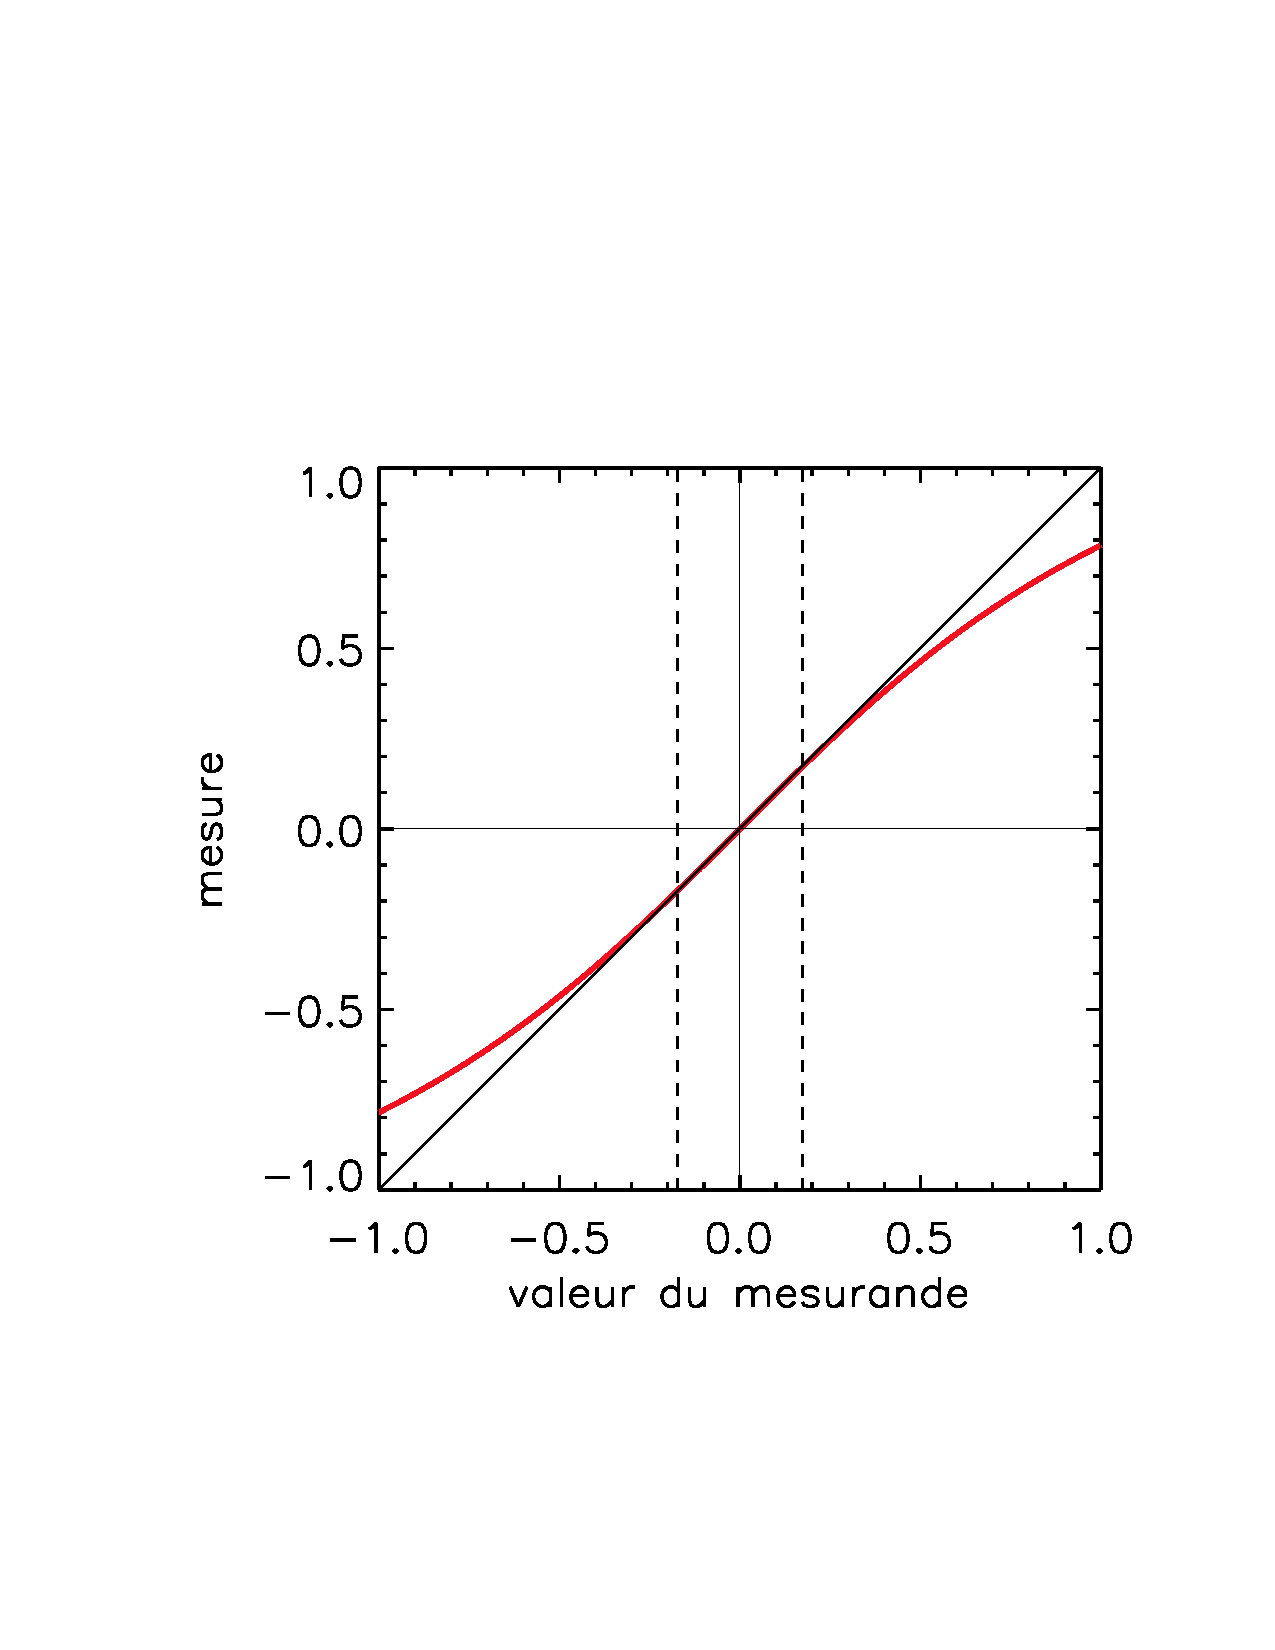
\includegraphics[width=7cm]{fig/nonlinearity.png}
\end{wrapfigure}
La plupart des instruments sont con�us pour fournir une relation lin�aire entre la valeur physique entr�e dans le syst�me et la valeur de sortie. Mais comme les syst�mes r�els ne sont jamais parfaitement lin�aires, ou alors seulement dans une certains �tendue de mesurage, une erreur est introduite � ce niveau, caract�ris�e par
\begin{equation}
\epsilon_\text{lin}\ [\%]=100\,\left|\frac{M-M_{\text{lin}}}{M}\right|
\end{equation}
o� $M_{\text{lin}}$ est la valeur donn�e par le syst�me, s'il �tait lin�aire. Dans la figure de droite est repr�sent�e la mesure brute d'un mesurande donn�e par un capteur, lin�aire uniquement dans une plage limit�e. Les deux traits tir�s verticaux montrent la plage dans laquelle l'erreur de non-lin�arit� est inf�rieure � 1 \%.

Il est important de noter que la non-lin�arit� n'est pas forc�ment un probl�me : si elle est connue, et bien mod�lis�e, il est toujours possible de la supprimer en corrigeant la mesure brute. Par exemple, dans le cas repr�sent� ici, la non lin�arit� se mod�lise tr�s bien avec une fonction arc-tangente. Il est donc possible de corriger la mesure brute en lui appliquant la fonction inverse de l'arc-tangente, c-�-d la tangente, tout simplement :
$$
\text{mesure brute}=\tan^{-1}(\text{valeur exacte})\ \ \text{d'o�}\ \ \text{valeur exacte}=\tan{(\text{mesure brute})}
$$

%..........................................
\subsection{Erreur de sensibilit�}
%..........................................

Dans la situation o� la mesure est r�alis�e � l'aide d'un capteur, il faut encore passer par la courbe d'�talonnage de ce dernier pour d�terminer la mesure dans l'unit� qui nous int�resse (par exemple dans le cas du thermocouple la tension est transform�e en une temp�rature). Si le syst�me est lin�aire, une erreur dans l'application du facteur de transformation (ou gain ou sensibilit�), pour une raison quelconque (parce que le gain est mal connu, par exemple) engendre ce que l'on appelle une erreur de sensibilit�.

%..........................................
\subsection{Erreur due � la r�solution de l�instrument}
%..........................................

La r�solution $\rho$ d'un instrument (les intervalles entre les graduations ou l'affichage sur l'�cran) est forc�ment toujours limit�e. Or, la mesure sera toujours affich�e � la valeur la plus proche possible que peut donner l'affichage. Par exemple si la valeur exacte du mesurande est 1.234 et que $\rho=0.1$ alors la valeur lue ou affich�e sera 1.2. Cette erreur d'arrondi peut au maximum �tre �gale � la moiti� de la r�solution, donc,
\begin{equation}
\epsilon_{\text{res}}=\pm\,\rho\,/\,2
\end{equation}

%..........................................
\subsection{Grandeurs d'influence externes}
%..........................................

Le syst�me peut, lors de son utilisation, �tre soumis � l'influence perturbatrice d�autres grandeurs physiques que celles du mesurande, dont les variations peuvent modifier la mesure, et qui sont impossibles � distinguer de celle due � l�action du mesurande. Les principales grandeurs d�influence sont les suivantes (la liste n'est pas exhaustive) :
\begin{description}
\item[la temp�rature,] qui a des effets �lectriques, m�caniques, g�om�triques (dilatation);
\item[la pression,] qui a un effet m�canique;
\item[l�acc�l�ration et les vibrations,] qui g�n�rent d�formations et contraintes;
\item[l�humidit�,] qui a un effet sur les constantes di�lectriques, la r�sistivit�, l'isolation;
\item[le champ �lectro-magn�tique,] qui g�n�re une force �-m et agit sur la r�sistivit�;
\item[la tension d�alimentation de l'instrument,] qui peut varier en amplitude et en fr�quence.
\end{description}
On cherchera � r�duire au maximum non seulement l'amplitude mais aussi et surtout la variation temporelle des grandeurs d'influence. En effet, si ces derni�res sont stables, les erreurs engendr�es seront constantes, donc syst�matiques, et il sera toujours possible de les identifier lors du processus d'�talonnage~: on verra dans ce cas que la courbe de d'�talonnage sera additionn�e d'une valeur syst�matique non nulle, alors que le mesurande est nul: on en d�duira qu'il existe une erreur syst�matique dues � des grandeurs d'influence, qu'il suffira de soustraire des mesures.

En revanche, si les grandeurs d'influence sont d'amplitude variable dans le temps, et de mani�re al�atoire et inconnue, alors il ne sera pas possible de s'affranchir de leur effet. Il conviendra alors de minimiser leur impact (par exemple, refroidissement stabilis� de l'appareil de mesure si la temp�rature est une grandeur d'influence critique), puis en dernier ressort d'estimer leur effet afin d'en tenir compte dans l'estimation de l'incertitude de la mesure.

%------------------------------------------
\section{Erreur et incertitude}
%------------------------------------------

\begin{wrapfigure}[10]{r}[6pt]{6cm}
   \centering
   \vspace{-5.5mm}
   \includegraphics[width=6cm]{fig/errinc.pdf}
\end{wrapfigure}
Insistons encore une fois sur la diff�rence fondamentale entre ces deux notions. \textbf{L�erreur de mesure} est d�finie comme la diff�rence entre la valeur mesur�e et la valeur vraie qui reste inconnue. On ne connait jamais la valeur de l'erreur, ni son signe, en revanche on peut estimer sa valeur absolue, en effectuant un �talonnage, et/ou un grand nombre de mesures. \textbf{L�incertitude de mesure} d�crit une r�gion \textbf{autour} de la valeur mesur�e dans laquelle on estime que se trouve la vraie valeur de l'observable.

L'incertitude est un nombre que l'on calcule, � partir de la connaissance de la statistique des erreurs. Elle peut �tre annonc�e de deux mani�res~:
\textbf{absolue}, auquel cas elle a la m�me unit� que la grandeur mesur�e, ou \textbf{relative} et se ramener � la valeur moyenne de l'observable, auquel cas elle est sans dimension et est g�n�ralement donn�e en \% de la valeur moyenne. Quoi qu'il en soit,
\begin{center}
\fbox{\begin{minipage}{14cm}\textbf{Une mesure sans indication d'incertitude est une mesure pratiquement inutile. On s'attachera donc � d�terminer l'incertitude avec le m�me soin que celui apport� � la prise de mesure elle-m�me.}\end{minipage}}
\end{center}

\begin{wrapfigure}[10]{r}[6pt]{7cm}
   \centering
   \vspace{-5mm}
   \includegraphics[width=7cm]{fig/errbar.pdf} 
   \caption{Graphique de donn�es exp�rimentales avec barres d'erreur.}
   \label{fig:errbar}
\end{wrapfigure}
Sur un graphique de donn�es exp�rimentales, l'incertitude de mesure sera d�crite � l'aide de barres d'erreur, comme en Fig.~\ref{fig:errbar}.

%------------------------------------------
\section{Comment annoncer un r�sultat ? les chiffres significatifs}
%------------------------------------------

L'incertitude est une grandeur que l'op�rateur du mesurage a la responsabilit� d'estimer, afin d'�tre indiqu�e avec la valeur de la mesure. L'incertitude n'est cependant elle-m�me rien d'autre qu'une valeur approximative ! car il faudrait une infinit� de mesures, et une connaissance absolue des caract�ristiques de l'instrument de mesure pour pouvoir �valuer avec pr�cision l'erreur probable commise de la mesure.

Par cons�quent, lorsque l'on annonce la valeur de l'incertitude, il n'y a aucun sens � donner trop de chiffres significatifs, en tout cas il ne sera pas utile d'aller trop en dessous de ce que contient l'estimation de l'incertitude. Admettons par exemple que la valeur d'une mesure soit $M=9.876543$ et que l'incertitude estim�e, dans la m�me unit�, soit $E=0.004321$. On arrondira en g�n�ral l'incertitude � 1 ou 2 chiffres significatifs, soit $E=0.004$ ou $0.0043$, et on arrondira la valeur de $M$ � la plus petite d�cimale associ�e � l'erreur $E$, soit � $10^{-3}$ ici. On �noncera donc le r�sultat de la mani�re suivante ~:
$$
M=9.877\pm0.004\ \ \text{[unit�]}
$$
Si cela est requis, il faudra encore donner le niveau de confiance de l'intervalle d'incertitude,
$$
M=9.877\pm0.004\ \ \text{[unit�], � 95 \%}
$$
Ecrire par exemple que $M=9\pm0.0042$ ou $M=9.876543\pm0.004$ est assez absurde. En revanche, �crire $M=9.876543\pm0.004321$ est acceptable, bien qu'inutile, car comme on l'a dit, $E$ est aussi entach� d'erreurs. Mais la discussion de ce type de probl�me nous entrainerait bien au-del� des objectifs de ce cours...

%------------------------------------------
\section{Erreurs syst�matiques et al�atoires : d�finitions}
%------------------------------------------

L�incertitude comprend les effets d�erreurs \textbf{syst�matiques} et d'erreurs \textbf{al�atoires}, qui d�pendent de l'exactitude et de la r�solution de l�instrument.

\textbf{L�erreur syst�matique} $\epsilon_s$ est la moyenne qui r�sulterait d�un nombre \textbf{infini} de mesurages du m�me mesurande, effectu�s dans des conditions de r�p�tabilit�, \textbf{moins} la valeur vraie du mesurande - Fig.~\ref{fig:eseea}. En g�n�ral, et � moins que l�instrument ne puisse �tre consid�r� d�une pr�cision parfaite, l�erreur syst�matique et ses causes ne peuvent �tre connues qu�en partie. Les effets des erreurs syst�matiques, quand ils ne peuvent pas �tre corrig�s, sont �valu�s d�apr�s l�exp�rience acquise ou d�apr�s d�autres informations.

\textbf{L�erreur al�atoire} $\epsilon_a$ est d�finie comme le r�sultat d�un \textbf{seul} mesurage (r�sultat individuel, Fig.~\ref{fig:eseea}) moins la \textbf{moyenne} d�un nombre infini de mesurages, effectu�s dans des conditions de r�p�tabilit� absolue. Comme on ne peut faire qu�un nombre limit� (fini) de mesurages, il n'est pas possible de d�terminer avec une pr�cision arbitrairement petite la moyenne des mesurages, et de fait, l'erreur al�atoire est elle-m�me sujette � une incertitude... L'amplitude des \textbf{erreurs al�atoires} peuvent cependant �tre �valu�es � partir de la statistique des r�sultats de s�ries de mesurages (voir le chapitre d'analyse de donn�es).

A ces deux erreurs peuvent s�ajouter les \textbf{erreurs grossi�res}, dues � des conditions anormales ou � des fautes techniques, et qui se manifesteront g�n�ralement par des valeurs absurdes, consid�rablement diff�rentes de toutes les autres valeurs.
\begin{figure}[t]
   \centering
   \includegraphics[width=14cm]{fig/errsysale.pdf} 
   \caption{Erreurs syst�matiques et al�atoires.}
   \label{fig:eseea}
\end{figure}

%..........................................
\section{Traitement des erreurs syst�matiques}
%..........................................

\subsection{Erreurs syst�matiques connues}

Les erreurs syst�matiques connues d'une mesure sont des grandeurs pouvant �tre d�termin�es tant du point de leur intensit� que de leur signe. Les normes (ex. DIN1319) fournissent d'autres d�signations telles que : erreurs syst�matiques avec signe connu, erreurs syst�matiques pures, erreurs corrigibles. Un r�sultat peut �tre corrig� des erreurs syst�matiques connues. \textbf{Lorsque la correction a �t� effectu�e, les erreurs syst�matiques connues ne font plus partie de l'indication d'incertitude de mesure}. Voici quelques exemples d'erreurs syst�matiques connues:
\begin{itemize}\itemsep2pt
\renewcommand{\labelitemi}{$\bullet$}
\item Une cale-�talon plus longue de 0.7 $\mu$m que la valeur nominale indiqu�e;
\item Une mesure de longueur effectu�e � une temp�rature de 25$^{\circ}$C au lieu de la temp�rature de r�f�rence de 20$^{\circ}$C, produisant une erreur syst�matique � la suite de la dilatation thermique de l'objet;
\item Un palmer qui poss�de des touches de palpage pr�sentant une usure mesurable;
\item Le tachym�tre d'une voiture qui pr�sente une indication de 5 km/h trop �lev�e dans une certaine plage;
\item Un voltm�tre dont on a v�rifi� qu�il poss�de un facteur d'amplification erron� ou indique une valeur trop �lev�e de 0.1 V dans toutes ses mesures.
\end{itemize}

\subsection{Erreurs syst�matiques inconnues}

Les erreurs syst�matiques inconnues sont g�n�ralement dues � des impr�cisions des instruments : celles-ci sont normalement d�finies en termes de valeurs (ou tol�rances) maximums, souvent avec le signe $\pm$. Il se peut que ces erreurs soient constantes dans une s�rie de mesures avec un �quipement particulier, mais on ne conna�t \textit{ni} leur valeur \textit{ni} leur signe. On d�finit souvent les erreurs syst�matiques inconnues comme des \textbf{erreurs de tol�rance}.

Les m�thodes pour prendre en compte les erreurs syst�matiques inconnues dans un calcul global d�incertitude font l�objet dՎtudes et de controverses depuis pr�s de 200 ans, et le sujet reste controvers� encore aujourd�hui.

Une approche fr�quemment utilis�e est la m�thode \textit{ISO Guide to the Expression of Uncertainty in Measurement (GUM)}. L�id�e de la m�thode GUM est de � transformer � les erreurs syst�matiques inconnues en erreurs al�atoires, en postulant une distribution statistique ad hoc, g�n�ralement rectangulaire.

%..........................................
\section{Traitement des erreurs al�atoires}
%..........................................

On distingue deux types d'erreurs al�atoires: de type dit A et de type dit B\footnote{La d�nomination type A ou B se r�f�re au \textit{ISO Guide to the Expression of Uncertainty in Measurement} - la m�thode GUM} :
%\begin{description}
%\item[Type A] Les erreurs al�atoires dont la valeur peut �tre estim�e par des m�thodes statistiques;
%\item[Type B] Les erreurs syst�matiques inconnues � converties � en erreurs pseudo-al�atoires et qui demandent pour leur �valuation la prise en compte additionnelle d�aspects non-statistiques tels que les caract�ristiques et tol�rances techniques de l�instrument, la pr�cision et fiabilit� de lՎtalonnage, l�exp�rience de l�op�rateur, etc..
%\end{description}

\subsection{Erreurs al�atoires de type A - �valu�es par des m�thodes statistiques}

Ces erreurs sont celles qui dues � des fluctuations des conditions environnementales (au sens large, ce qui inclut l�op�rateur et l�instrument) au cours de la mesure, et � la fluctuation �ventuelle du mesurande, lorsque celui-ci est de nature variable (param�tres atmosph�riques, par exemple). Le signe et l'amplitude instantan�e de cette erreur sont par cons�quent inconnus. Lors de mesures r�p�t�es au cours d'une s�rie, on trouve que
\begin{enumerate}
\item ces erreurs al�atoires fluctuent de mani�re impr�visible par rapport � une valeur moyenne;
\item mais que l�incertitude sur la moyenne diminue avec le nombre de mesures, car en moyenne, les erreurs de type A se compensent. On montre au chapitre sur l'analyse de donn�es que l'erreur sur la moyenne diminue comme $1/\sqrt{N}$ o� $N$ est le nombre de mesures. Avec 10'000 mesures, on est donc 10 fois plus pr�cis qu'avec 100 mesures.
\end{enumerate}

\textbf{Le cours de m�trologie de l'office f�d�ral de m�trologie - METAS}, introduit les erreurs al�atoires de type A de la mani�re suivante~:
\begin{center}
\begin{minipage}{\textwidth}\sl
Lorsque les fluctuations d'une grandeur de mesure $X$ peuvent �tre d�crites par des m�thodes statistiques, on parle d'une estimation de type A de l'incertitude de mesure. La valeur de la grandeur ainsi que son incertitude-type seront d�termin�s par un ensemble de $n$ observations effectu�es dans des conditions de mesure semblables. Par exemple~:
\begin{itemize}\itemsep2pt
\renewcommand{\labelitemi}{$\circ$}
\item Lectures r�p�t�es de l'affichage fluctuant d'un instrument de mesure (analogique ou digital).
\item Mesures r�p�t�es apr�s un nouveau r�glage de l'instrumentation de mesure: estimation de l'exactitude du r�glage et de l'influence de l'op�rateur.
\end{itemize}
\end{minipage}
\end{center}
\rm
On quantifie ces erreurs al�atoires, qui ont souvent une distribution gaussienne, par leur �cart-type\footnote{voir le chapitre d'analyse de donn�es}. Voici quelques exemples d'erreurs al�atoires de type A :
\begin{itemize}\itemsep2pt
\renewcommand{\labelitemi}{$\bullet$}
\item bruit d'instruments �lectroniques (amplificateurs) produisant des fluctuations du signal amplifi�,
\item influence de vibrations m�caniques sur l'instrument de mesure,
\item jeux dans les roulements d'arbres de dispositifs m�caniques complexes,
\item erreurs de lecture des graduations d'un microscope en raison d'une nettet� insuffisante,
\item fluctuation de la temp�rature ambiante � la suite d'un d�faut de r�gulation thermostatique ou par ouverture et fermeture r�p�t�e d'une porte du local de mesure. Une fluctuation de la temp�rature de l'objet � mesurer peut �galement intervenir � la suite d'un contact avec la main de l'op�rateur,
\item influence de la fluctuation al�atoire du champ �lectrique et magn�tique sur l'indicateur d'instruments de mesure �lectriques,
\item temps d'arriv�e al�atoire des photons dans un dispositif de comptage de photons.
\end{itemize}

\newpage

\subsection{Erreurs al�atoires de type B - �valu�es par des m�thodes non statistiques}

\textbf{Le cours de m�trologie de l'office f�d�ral de m�trologie - METAS}, introduit les erreurs al�atoires de type B de la mani�re suivante~:
\begin{center}
\begin{minipage}{\textwidth}\sl
Dans le cas o� la valeur estim�e x d'une grandeur X ne peut pas �tre d�termin�e � partir de la r�p�tition des mesures, l'incertitude-type u(x) doit �tre trouv�e � partir d'arguments scientifiques qui prennent en compte toutes les sources de fluctuation de la grandeur X. Dans cette �valuation, les sources d'information suivantes peuvent par exemple �tre utilis�es:
\begin{itemize}\itemsep2pt
\renewcommand{\labelitemi}{$\circ$}
\item Mesures pr�c�dentes
\item Exp�rience ou connaissance du comportement et des propri�t�s des instruments et composantes du syst�me de mesure
\item Sp�cifications des fabricants
\item Donn�es des certificats d'�talonnage
\item Incertitude sur les valeurs de r�f�rence
\end{itemize}
\end{minipage}
\end{center}
\rm

Parmi de telles erreurs se trouvent, typiquement, les tol�rances des instruments de mesure. Leur amplitude ainsi que leur signe au moment d�une mesure d�termin�e sont inconnus. Toutefois leur pr�sence ainsi que l'intensit� maximale (tol�rance) est connue. Dans le cadre de mesures r�p�t�es dans une s�rie de mesures, il se peut que ces erreurs inconnues aient toujours la m�me valeur et le m�me signe. Le probl�me est que cette valeur ainsi que ce signe sont inconnus : on ne conna�t en g�n�ral que la valeur maximale. \textbf{En fait, les erreurs syst�matiques inconnues, introduites ci-dessus, peuvent tout � fait �tre consid�r�es comme des erreurs al�atoires de type B !}

Voici quelques exemples d'erreurs de type B:
\begin{itemize}\itemsep2pt
\renewcommand{\labelitemi}{$\bullet$}
\item La r�solution d�un affichage num�rique;
\item Un palmer qui poss�de une tol�rance connue de 0.3 $\mu$m. On ne sait cependant pas si l'erreur est de -0.3 $\mu$m ou +0.3 $\mu$m;
\item Le cas o�, lors d'une mesure de longueur, la temp�rature de l'objet n'est pas mesur�e. On sait cependant qu'au cours des mesures, la temp�rature se trouvait dans la tol�rance de $\pm1^{\circ}$C par rapport � la temp�rature de r�f�rence de 20$^{\circ}$C;
\item Une jauge qui poss�de une grandeur nominale de 30.000 mm et une indication de tol�rance de $\pm 1\mu$m.
\end{itemize}
On remarquera que les erreurs de type B se distinguent des erreurs de type A par le fait qu�elles ne peuvent pas �tre diminu�es en augmentant le nombre de mesures effectu�es: faire 10'000 mesures d'une tension �lectrique ne r�duira pas l'incertitude due � la r�solution de l'affichage du voltm�tre !

Les erreurs de ce type peuvent �tre d�termin�es ou estim�es de plusieurs mani�res, selon le cas~:
\begin{itemize}\itemsep2pt
\renewcommand{\labelitemi}{$\bullet$}
\item A partir des caract�ristiques de l'instrument donn�e par le fabriquant. Par exemple, si d'apr�s ce dernier, la lin�arit� d'un voltm�tre est de 0.1\% de la gamme de mesure de 300 V, il en r�sulte une erreur syst�matique inconnue de $\pm$0.3 V, � laquelle on associera une distribution rectangulaire\footnote{voir le cours � Analyse de donn�es en sciences exp�rimentales �};
\item Comparaison avec un instrument de mesure au moins dix fois plus pr�cis;
\item Calcul des tol�rances � partir des tol�rances m�caniques et des relations g�om�triques de l'instrument de mesure, par exemple en cas de dilatation thermique.
\end{itemize}

%..........................................
\section{Traitement des erreurs grossi�res}
%..........................................

Apr�s chaque s�rie de mesures, il faut encore d�tecter et �liminer les erreurs grossi�res. L'origine de ces derni�res doit aussit�t �tre �lucid�e de mani�re � ce que cette situation ne se reproduise plus au cours des s�ries de mesures suivantes. Si elles ne sont pas \textbf{�limin�es} elles peuvent influencer consid�rablement la valeur moyenne et l'�cart-type d'une s�rie de mesures.

Quelques exemples d'erreurs grossi�res :
\begin{itemize}\itemsep2pt
\renewcommand{\labelitemi}{$\bullet$}
\item Les premi�res valeurs d'une s�rie de mesures peuvent �tre erron�es si l'appareil de mesure ne fournit des valeurs fiables qu'apr�s un certain temps d'�chauffement;
\item Fausse lecture d'une mesure, par exemple par une erreur de virgule ou du facteur x10, x100 affich�;
\item Les �l�ments d'une cha�ne de mesure ne sont pas correctement adapt�s en imp�dance;
\item Tension d'alimentation fausse ou fluctuante;
\item Choc contre l'instrument de mesure au cours du mesurage;
\item L'appareil utilis� est d�fectueux en raison d'une chute ant�rieure;
\item Mauvaise manipulation de l'appareil en raison de la m�connaissance du mode d'emploi de ce dernier.
\end{itemize}

%\input{src/solutions.tex} (missing figures there)

\backmatter

\listoffigures
%\listoftables

\input{src/colophon}


\end{document}
